%%%%%%%%%%%%%%%%%%%%%%%%%%%%%%%%%%%%%%%%%%%%%%%%%%%%%%%%%%%%%%%%%%%%%%%%
%                                                                      %
%     File: Thesis_SPI.tex                        %
%     Tex Master: Thesis.tex                                %
%                                                                      %
%     Author: Carlos A. Rodrigues                         %
%     Last modified : 15 Abril 2013                         %
%                                                                      %
%%%%%%%%%%%%%%%%%%%%%%%%%%%%%%%%%%%%%%%%%%%%%%%%%%%%%%%%%%%%%%%%%%%%%%%

\chapter{SPI}
\label{chapter:spi}

% pdf sd_spi
O nosso \acrshort{soc} tem disponível uma memoria principal voatil ou seja sempre que a memoria é desligada da fonte de alimentação perde a informação contida nela. Então é necessário ter disponível no \acrshort{soc} uma outra memoria que não seja voatil como um cartão \acrlong{sd}, uma EEPROM, para se poder guardar o programa, que será carregado para a memoria principal sempre que o \acrshort{soc} for inicializado ou seja alimentado. Optou-se pela utilização de um cartão \acrshort{sd} por permitir uma fácil substituição em qualquer local que esteja aplicado o \acrshort{soc} a trabalhar, estando planeado que estagia a trabalhar em locais de difíceis acessos. O cartão \acrshort{sd} é possível ligar-se por barramento \acrshort{spi}, como se pode ver na tabela \ref{table:pin_sd_card} e a correspondência entre os pinos na figura \ref{fig:cartao_SD} que se encontra ao lado.

\textcolor[rgb]{1,0,0}{melhorar a posição disto}

  \begin{minipage}{\textwidth}
  \begin{minipage}[b]{0.20\textwidth}
    \centering
    \includegraphics[width=1\textwidth]{Figures/sd_card.pdf}
    \captionof{figure}{Cartao SD}
    \label{fig:cartao_SD}
  \end{minipage}
  \hfill
  \begin{minipage}[b]{0.99 \textwidth}
    \centering
    \begin{tabular}{c | c | c| c}\hline
      Pinos SD & Nome(SD) & Nome (SPI) & Descrição  \\ \hline
        1 & CS & SS & Selectiona o cartão \\
        2 & DI & MOSI & Entrada de dados\\
        3 & VSS & -- & Tensão de alimentação(massa) \\
        4 & VDD & -- & Tensão de alimentação \\
        5 & SCLK & SCLK & Clock \\
        6 & VSS & -- & Tensão de alimentação(massa) \\
        7 & DO & MISO & Saida de dados\\
        8 & RSV & -- & Reservado  \\
        9 & RSV & -- & Reservado \\ \hline
      \end{tabular}
      \captionof{table}{Relação pinos do cartão SD SPI}
      \label{table:pin_sd_card}
    \end{minipage}
  \end{minipage}

Como foi dito \ref{section:spi} o \acrshort{spi} é um barramento de comunicação utilizado em casos onde é necessário uma comunicação com a velocidade de transferências elevada, como é neste caso. O barramento é constituído por 3 linhas de comunicação mais uma por cada escravo que esteja ligado a mestre como se pode ver na figura \ref{fig:ligacoesSPI}, neste caso como tem três escravos têm 3 linhas mais 3 linhas de selecção de escravo. A linha que seleciona o escravo é a linha \acrshort{ss} esta é seleciona o escravo quando tem um valor lógico de '0'. Apenas o escravo que está selecionado lé e/ou escreve no barramento, como se trata de barramento full-duplex têm disponível uma linha de leitura para o escravo \acrshort{mosi}  e outra de escrita do escravo \acrshort{miso}. Ainda existe mais uma linha de sincronização com um sinal de clock \acrshort{sclk}. Todas as linhas do barramentos com as excepção da \acrshort{ss} são partilhadas por todos os escravos, a linha \acrshort{ss} como se trata de uma linha de selecção de escravo cada escravo tem a sua linha independente. Para se efetuar comunicação o mestre SPI seleciona com qual escravo quer comunicar, dependendo do escravo com que está a comunicar enviar uma ou mais palavras de 8 bits na linha \acrshort{mosi} sincronizado com o sinal de clock que se encontra na linha \acrshort{sclk}, posteriormente o mestre necessita de transmitir mais sinais de clock para o escravo, para este poder transmitir os dados pedidos pelos mestres na linha \acrshort{miso}.

\begin{figure}[!htb]
  \centering
  \includegraphics[width=0.50\textwidth]{Figures/SPI.png}
  \caption[Protocolo SPI]{Esquematico do sistema de comunicação SPI, com 1 master e vários escravos"tirou do wiki".}
  \label{fig:ligacoesSPI}
\end{figure}

\section{Mestre SPI}

A comunidade OpenRISC já tinha disponível um core de mestre \acrshort{spi} com uma interface Wishbone disponível para ligação ao \acrshort{soc}. Porém este core apenas realizava corretamente escritas para o escravo, não efetuando qualquer leitura de dados enviada pelo escravo. Sendo uma parte indispensável para o objectivo que seria pretendido para o core de \acrshort{spi}, como foi dito em cima seria efetuar leituras de uma memoria de um cartão \acrshort{sd} para efetuar o carregamento do programa para a memoria principal.

Na figura \ref{fig:diagrama_SPI_master} pode ser visto o fluxo de dados dentro do core mestre de SPI. Quando se pretende enviar uma palavra para o escravo esta é recebida pelo cores vindo da interface Wishbone que se encontra ligada ao processador do \acrshort{soc}, é guardada na \acrshort{fifo}, com uma tamanho de 4 palavras, que contem as palavras que serão enviadas para o escravo, na figura tem o nome de \acrshort{fifo} IN. Quando o modelo que faz a serialização se encontra parado e tem disponível uma palavra para enviar na \acrshort{fifo}. O modelo vai buscar a palavra à \acrshort{fifo} e começa a gerar clocks ao mesmo tempo que serializa a palavra e a enviar bit a bit para o escravo pela linha \acrshort{mosi}.

Quando se pretende receber dados do escravo, o modelo de desserialização recebe essa informação e se a \acrshort{fifo} que recebe as palavras vindas do escravo, na figura com o nome de \acrshort{fifo} OUT, não estiver cheia, começa a gerar clock's. O modelo recebe bit a bit a palavra do escravo na linha \acrshort{miso}, quando receber a palavra toda deixa de gerar clocks e enviar a palavra para a \acrshort{fifo}. Em seguida a palavra será enviada da \acrshort{fifo} para o processador pela interface Wishbone. Visto que se trata de um barramento full-duplex quando se encontra a enviar dados para o escravo, o mestre também lé a linha \acrshort{miso} e guarda a palavra da \acrshort{fifo}. No caso destes dados forem lixo é necessário ter em atenção se os dados não forem removidos da \acrshort{fifo} quando se for efectuar a primeira leitura podemos estar a ler lixo. 

\begin{figure}[!htb]
  \centering
  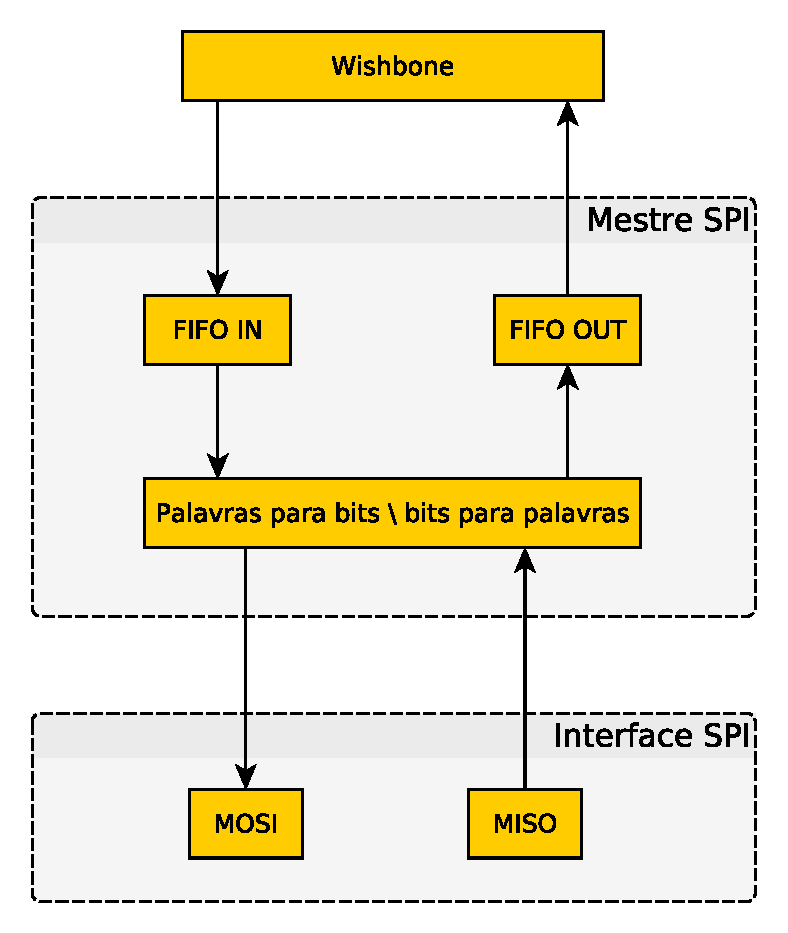
\includegraphics[width=0.50\textwidth]{grafos/diagrama_SPI_master.pdf}
  \caption[Fluxo dos dados dentro do core mestre SPI]{Fluxo dos dados dentro do core mestre SPI}
  \label{fig:diagrama_SPI_master}
\end{figure}

Na tabela \ref{table:sinais_SPI_master} temos todos os sinais do core mester de \acrshort{spi} com uma pequena descrição, os primeiros 10 sinais correspondem à interface Wishbone que é ligado ao multiplexer wishbone de dados á semelhança dos cores de uart e de gpio como se pode ver na figura \ref{grafos:wishbone}. Os ultimos quatros sinais correspondem a barramento \acrshort{spi} para serem ligados ao escravo.

\begin{table}[h!]
  \begin{center}
    \begin{tabular}{|C{2cm}|c|c|c|}
      \hline
       Interface & Nome & direcção & Descrição \\
      \hline \hline
      \multirow{10}{*}{Wishbone} & clk\_i & input & Clock, Recebido pelo Wishbone. \\
      \cline{2-4}
      & rst\_i & input & Reset, renicia o core quando se encontra no valor logic "1".\\
      \cline{2-4}
      & cyc\_i & input & \\
      \cline{2-4}
      & stb\_i & input & \\
      \cline{2-4}
      & adr\_i & input & Endereço do registo onde se pretende ler ou escrever no core.\\
      \cline{2-4}
      & we\_i & input & Bit de selecção de escrita.\\
      \cline{2-4}
      & dat\_i & input & Recepção de dados por parte do processador.\\
      \cline{2-4}
      & dat\_o & output & Envio de dados para o processador.\\
      \cline{2-4}
      & ack\_o & output & bit que informação o processador a recepção do comando pelo core.\\
      \cline{2-4}
      & inta\_o & output & bit de interrupção. \\
      \hline \hline
      \multirow{4}{*}{SPI} & sck\_o & output & Clock do protocolo de comunicação SPI.\\
      \cline{2-4}
      & ss\_o & output & Faz a selecção do escravo que se pretende ler ou escrever.\\
      \cline{2-4}
      & mosi\_o & output & envio de dados para o escravo (master Out Slave In).\\
      \cline{2-4}
      & miso\_i & input & recepecção de dados do escravo (master Out Slave In).\\
      \hline
    \end{tabular}
  \end{center}
  \caption[Tabela de sinais do core SPI master]{Tabela de sinais da interface SPI master}
  \label{table:sinais_SPI_master}
\end{table}

A tabela \ref{table:registos_SPI_master} é uma descrição dos registos do mestre \acrshort{spi} com uma pequena descrição de cada registo e o seu Offset. 

\begin{table}[h!]
  \begin{center}
    \begin{tabular}{|c|c|c|c|}
      \hline
      Nome & leitura/escrita & Descrição & Offset End. \\
      \hline \hline
      Registo de controlo & escrita e leitura &  & 0X00 \\
      \hline
      Tipo de leitura & escrita  & selectiona o tipo de leitura que é pretendida no SPI & 0X01 \\
      \hline
      Registo de estado & leitura & disponibliza várias informações do estado do core & 0X01 \\
      \hline
      Leitura de dados & leitura & leitura dos dados recebidos pelo SPI & 0X02 \\
      \hline
      Escrita de dados & escrita & escrita dos dados a enviar pelo SPI & 0X02 \\
      \hline
      Ext.registo de controlo & escrita e leitura & & 0X03 \\
      \hline
      selecção do escravo & escrita e leitura & seleciona o escravo que se pretende escrever ou ler & 0X04 \\
      \hline
    \end{tabular}
  \end{center}
  \caption[Tabela de registo do core SPI master]{Tabela de registos da interface SPI master}
  \label{table:registos_SPI_master}
\end{table}

O core mestre de \acrshort{spi} disponibiliza o modo de escrita que já se encontrava funcional, ficando a disponibilizar também o modo de leitura de dados que não se encontrava totalmente funcional. Esta leitura que a vou chamar de simples era feita apenas quando o era pedida pela processador ou seja, o processador pedia para ler uma palavra ao core, ai ele realizava a leitura no core. Este tipo de leitura perde-se bastante tempo porque o processador tinha de ficar a espera o core efectua-se a leitura ao escravo e que este o respondesse com a palavra, principalmente se pensarmos para que tipo de funcionalidade foi adicionado, para efetuar leitura sucessivas e posições de memorias sequenciais. Então pensei como poderia diminuir o tempo em que o processador tivesse a espera da resposta do core de forma transparante para ele. A solução encontrada é existir dois modos de leitura, um modo simples descrito em cima e outro modo em brust. Quando se efectua uma leitura é necessário identificar o tipo de leitura ao core, isto é feito no registo com o offset 0x01 como se pode ver na tabela \ref{table:registos_SPI_master} se escrevemos a palavra 0x02 é uma leitura simples, se for 0x01 é uma leitura brust. A principal diferença entre os dois modos de leitura é que o core na leitura simples vai pedir dados escravo após cada pedido pelo processador, na leitura em brust o core faz pedidos de dados sucessivos ao escravos até a \acrshort{fifo} OUT ficar cheia, ou seja não espera que o processador peça dados. Este tipo de leitura só mostra vantagem quando são leitura sucessivas de vários dados sucessivos como por exemplo a carregar o programa na memoria principal, \textcolor[rgb]{0,1,0}{como se pode ver nas figuras XXXX por imagem das ondas a comprar o tempo.}

\section{escravo SPI}

dizer que foi desenhado desde o inicio.

por um diagrama de blocos de como circula a informa\c{c}\~ao dentro do meu modelo de SPI. fazer uma descri\c{c}\~ao do funcionamento com uma descri\c{c}ao do fluxo de dados.
\begin{figure}[!htb]
  \centering
  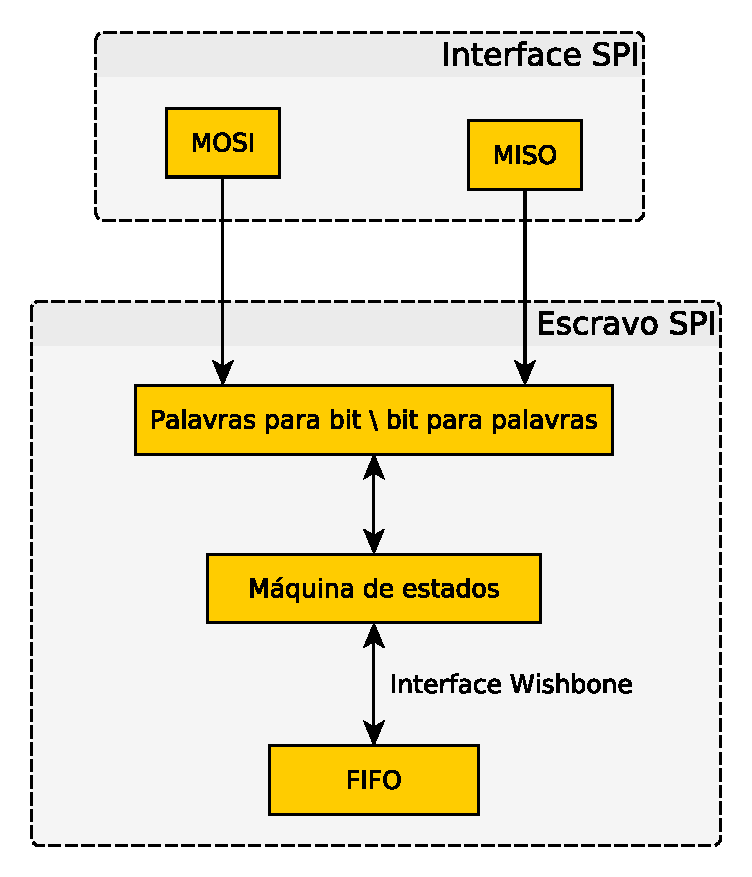
\includegraphics[width=0.50\textwidth]{grafos/diagrama_SPI_slave.pdf}
  \caption[Fluxo de dados dentro do core SPI escravo]{Fluxo dos dados dentro do core SPI escravo}
  \label{fig:diagrama_SPI_slave}
\end{figure}

por a tabela de sinais da interface de SPI (sinais de entrada e saida)
\begin{table}[h!]
  \begin{center}
    \begin{tabular}{|c|c|c|}
      \hline
      Nome & direcção & Descrição \\
      \hline \hline
      clk\_i & input & Clock, Recebido pelo Wishbone. \\
      \hline
      rst\_i & input & Reset, renicia o core quando se encontra no valor logic "1".\\
      \hline
      sck\_o & input & Clock do protocolo de comunicação SPI.\\
      \hline
      ss\_o & input & selectiona se é o escravo pretendido\\
      \hline
      mosi\_o & input & recepecção de dados do master (masterOut SlaveIn).\\
      \hline
      miso\_i & output & envio de dados para o master (masterOut SlaveIn).\\
      \hline
    \end{tabular}
  \end{center}
  \caption[Tabela de sinais SPI escravo]{Tabela de sinais da interface SPI escravo}
  \label{table:sinais_SPI_slave}
\end{table}

explicar o modo de funcionamento de esrita e de leitura.

explicar os 2 modos de funcionamento de esrita e de leitura que tem 2 modos.

\section{Diagramas temporais}

Em seguida temos os diagramas temporais com uma breve explicação do que se encontra em cada diagrama.

\subsection{Selecção de chip}

Na figura \ref{fig:ondas_SPI_S} estão ligados dois escravos ao mestre de \acrshort{spi}, por essa razão existes dois sinais de \acrshort{ss} cada um ligado apenas a uma escravo.
Como foi dito em cima o sinal de \acrshort{ss} é ativo em baixo, significa que o escravo está selecionado quando o seu sinal tem o valor lógico de '0'. No primeiro flanco positivo da figura \ref{fig:ondas_SPI_S} não se encontra qualquer um dos escravos selecionado, o escravo um é selecionado no primeiro flanco negativo e assim se mantem até ao segundo flaco negativo, o segundo escravo é selecionado no terceiro flanco negativo e desselecionado no quarto flanco negativo. Apenas o segundo e o quarto flanco positivo têm um escravo selecionado, o primeiro e o segundo escravo correspondentemente. 

\begin{figure}[!htb]
  \centering
  \includegraphics[width=0.75\textwidth]{ondas/SPI_S.pdf} %0.5
  \caption[Diagrama temporal da selecção do escravo.]{Diagrama temporal da selecção do escravo.}
  \label{fig:ondas_SPI_S}
\end{figure}

\subsection{Dados}

Os dados transmitidos tanto pelo mestre ou pelo escravo são lidos nos flancos positivo.

\subsubsection{Envio de dados pelo mestre}

No caso do envio dos dados do mestre para o escravo estes são feitos pelo sinal \acrshort{mosi} como se pode ver na figura \ref{fig:ondas_SPI_Se}. O escravo apenas vai guardar os dados que forem enviados depois de ser selectionado, que so acontece após o segundo flaco positivo. Após o escravo ser selecionado os dados são lidos no flanco positivo do sinal de \acrshort{sclk}, nesta figura por exemplo as palavras são de 6 bits, a palavra recebida pelo escravo no exemplo da figura é 110100 na base binária.

\begin{figure}[!htb]
  \centering
  \includegraphics[width=1.00\textwidth]{ondas/SPI_Se.pdf} %0.5
  \caption[Diagrama temporal do envio de dados pelo mestre.]{Diagrama temporal do envio de dados pelo mestre.}
  \label{fig:ondas_SPI_Se}
\end{figure}

\subsubsection{Envio de dados pelo escravo}

Para o escravo enviar dados para o mestre, o mestre necessita de criar o sinal de clock em \acrshort{sclk} e o escravo só pode usar o sinal \acrshort{miso} quando se encontra selecionado. Como no envio de dados do mestre para o escravo, neste caso do envio de dados do escravo para o mestre os dados são lidos nos flancos positivos do sinal de clock gerado pelo mestre. A caso de exemplo a figura \ref{fig:ondas_SPI_Re} a palavra envida pelo escarvo é de apenas 6 bits, neste exemplo a palavra transferida pela o escravo é 010110 na base binária. 

\begin{figure}[!htb]
  \centering
  \includegraphics[width=1.00\textwidth]{ondas/SPI_Re.pdf} %0.5
  \caption[Diagrama temporal do envio de dados pelo escravo.]{Diagrama temporal do envio de dados pelo escravo.}
  \label{fig:ondas_SPI_Re}
\end{figure}
